\section{Result}

Our results are divided into two parts.
In the first part, we have our measurement made using our external benchmarking framework.
In the second part, we used the oscilloscope to compute the real context-switching time.

\subsection{Context switching measured by our framework}
The context switching time computed by our external benchmarking framework is displayed in the table \ref{tab:external-framework-measurement}.

\begin{table}[!ht]
  \centering
  \begin{tabular}{llll}
                        & \multicolumn{3}{c}{Time ($\mu$s)}                             \\ \cline{2-4} 
                        & \multicolumn{1}{c}{Mean} & Min  & \multicolumn{1}{c}{Max} \\ \cline{2-4} 
  Context switching time & 18.93                     & 15.62 & 40.26                    \\
  \end{tabular}
  \caption{Context switching time measured by our external benchmarking framework}
  \label{tab:external-framework-measurement}
\end{table}

\subsection{Context switching measured by the oscilloscope}
Using the oscilloscope, we compute the real context switching time in order to catch any overhead induce by our external benchmarking framework.
The table \ref{tab:external-oscilloscope-framework-measurement}.

The figure \ref{fig:external-framework-value-wave} shows the voltage of the GPIO used by our external benchmarking framework.

\begin{table}[!ht]
  \centering
  \begin{tabular}{llll}
                        & \multicolumn{3}{c}{Time ($\mu$s)}                             \\ \cline{2-4} 
                        & \multicolumn{1}{c}{Mean} & Min  & \multicolumn{1}{c}{Max} \\ \cline{2-4} 
  Context switching time & 14.87                     & 14.79 & 14.97                    \\
  Duration of task 1    & 1003                     & 1003 & 1003                    \\
  Duration of task 2    & 1003                     & 1003 & 1003                   
  \end{tabular}
  \caption{Context switching times and task durations measured with the oscilloscope Tektronix MSO 56 using our external benchmarking framework}
  \label{tab:external-oscilloscope-framework-measurement}
\end{table}

\begin{figure}[!ht]
  \centering
  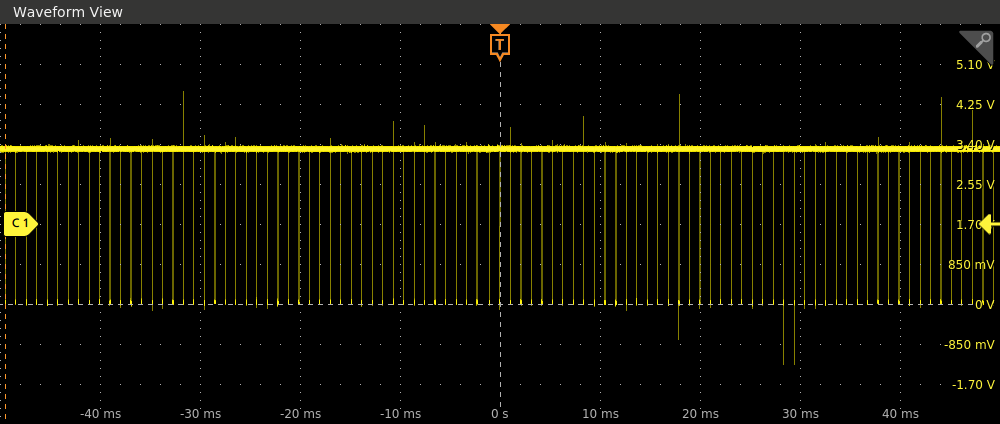
\includegraphics[scale=0.5]{assets/external-framework-value-wave.png}
  \caption{\label{fig:external-framework-value-wave}Voltage measurement of the GPIO used by the external benchmarking framework}
\end{figure}

\subsection{Discussion}

The first thing we can see is that our external benchmarking framework is much more precise that our internal benchmarking framework.
Even if the result does not match our excpectation, the results show an improvement.
We went from a measurement error with a factor of more than 500 to a measurement error with a factor less than 2.

Secondly, with the real context switching time measured at 14.87$\mu$s while our framework was on, our external benchmarking framework does not add an overhead.

In conclusion, our external benchmarking framework is more precise than our internal benchmarking framework and does not add an overhead to the real context switching time.